\documentclass[a4paper, 12pt]{article}
\usepackage{jipkg}

\title{X Facteur\\Dossier préliminaire au projet}
\author{Cléo \textsc{Daguin}, Léo \textsc{Massy} \& Quentin \textsc{Ribac}}
\date{\today}
\jihypersetup{X Facteur — Dossier préliminaire au projet}{Cléo DAGUIN, Léo MASSY \& Quentin RIBAC}

\begin{document}
\maketitle
\renewcommand{\contentsname}{Sommaire}
\tableofcontents
\newpage

\jisec{Équipe}
Notre équipe pour la réalisation du logiciel X Facteur est composée de :
\begin{description}
\item[Chef de projet] Quentin Ribac
\item[Acteur] Cléo Daguin
\item[Acteur] Léo Massy
\end{description}

\jisec{Enjeux du projet}
\jissec{Objectif du projet}
\jiimgsmp{fig:bete-a-cornes}{img/bete-a-cornes}{Bête à cornes pour X Facteur}

\jissec{Contexte}
La Poste a besoin d’un nouveau logiciel qui lui permettrait de calculer le chemin le plus court pour
ses facteurs, ce qui économiserait du carburant et du temps lors de leur distribution du courrier.

Notre partenaire sera un fournisseur de carte (tel que Google Maps ou Open Street Map).

\clearpage
\jisec{Principaux éléments de l’analyse fonctionnelle}
\jissec{Besoins fonctionnels}
\begin{itemize}
\item affichage de la carte
\item algorithme de calcul du trajet le plus court
\item affichage du trajet
\item gestion des facteurs (nombre \& mode de déplacement)
\item gestion des colis (adresse de livraison \& type)
\end{itemize}

\jissec{Besoins non fonctionnels}
\begin{itemize}
\item la documentation utilisateur
\end{itemize}

\jissec{Contraintes}
\begin{itemize}
\item des rues sont à sens uniques
\item des rues sont réservées aux piétions
\item l’algorithme ne doit pas être trop lent au calcul du trajet
\item le nombre de facteur est variable
\item certains facteurs sont véhiculés et d’autres non
\item livrer un colis requiert un véhicule
\end{itemize}

\jissec{Exclusions}
\begin{itemize}
\item une seule carte
\item un seul centre de distribution duquel partent et où reviennent les facteurs
\end{itemize}

\jissec{Maquette}
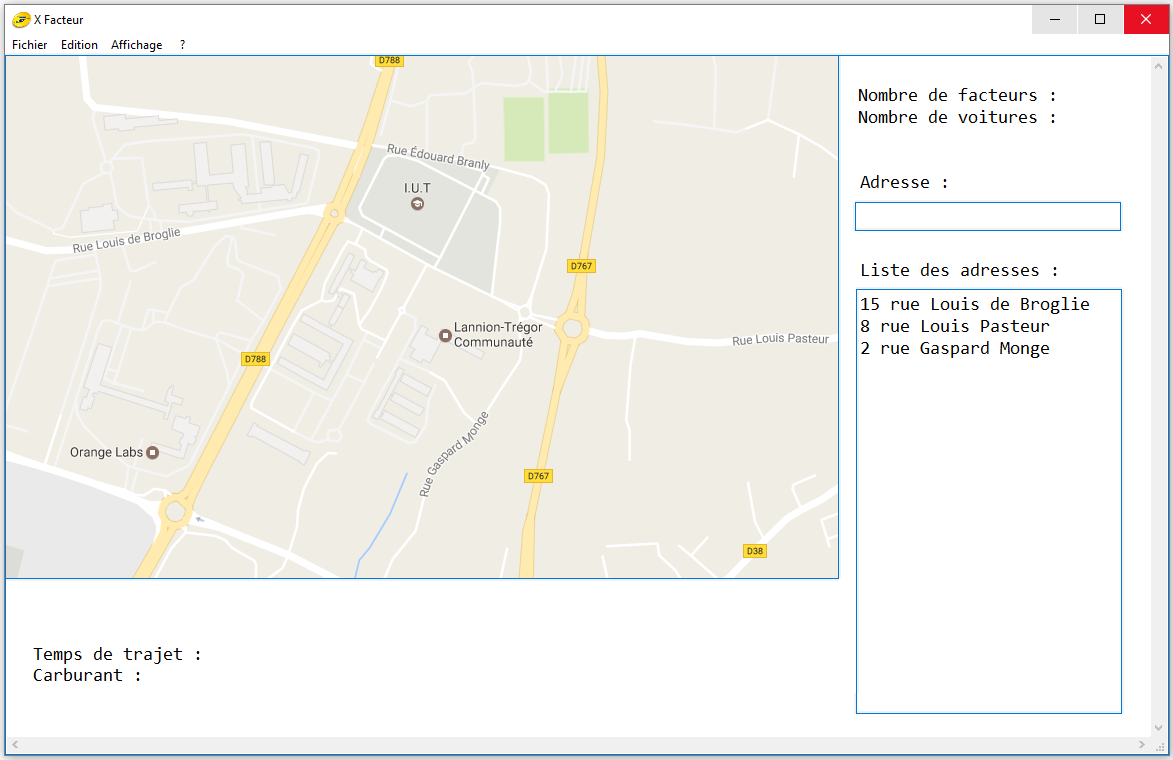
\includegraphics[width=0.8\textwidth]{img/maquette}

\clearpage
\jisec{Principaux risques}
\begin{itemize}
\item échouer dans la conception de l’algorithme
\item échouer dans la modélisation
\item échouer dans la recherche de ressources pour l’intégration de la carte
\end{itemize}

\jisec{Acteurs}
\begin{itemize}
\item facteurs
\item responsables de La Poste
\end{itemize}

\clearpage
\begin{multicols}{2}
\jisec{Diagramme des tâches (WBS)}
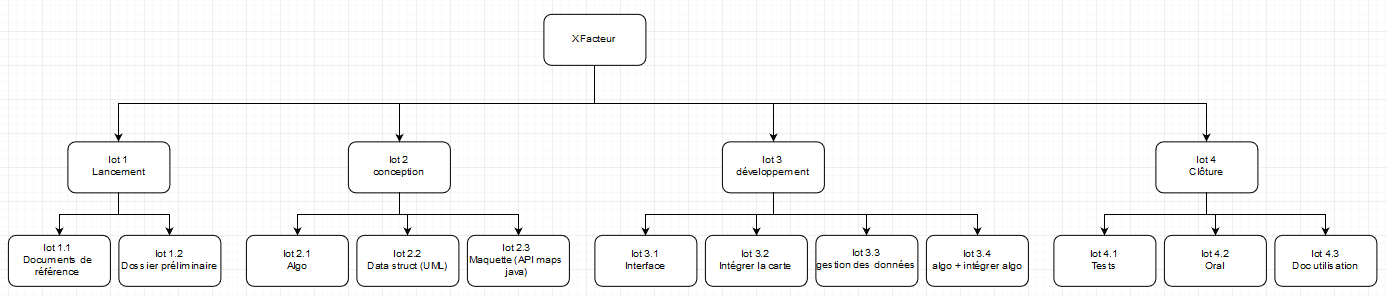
\includegraphics[angle=90, height=0.9\textheight]{img/diag-taches}
\columnbreak
\jisec{Diagramme des responsabilités (OBS)}
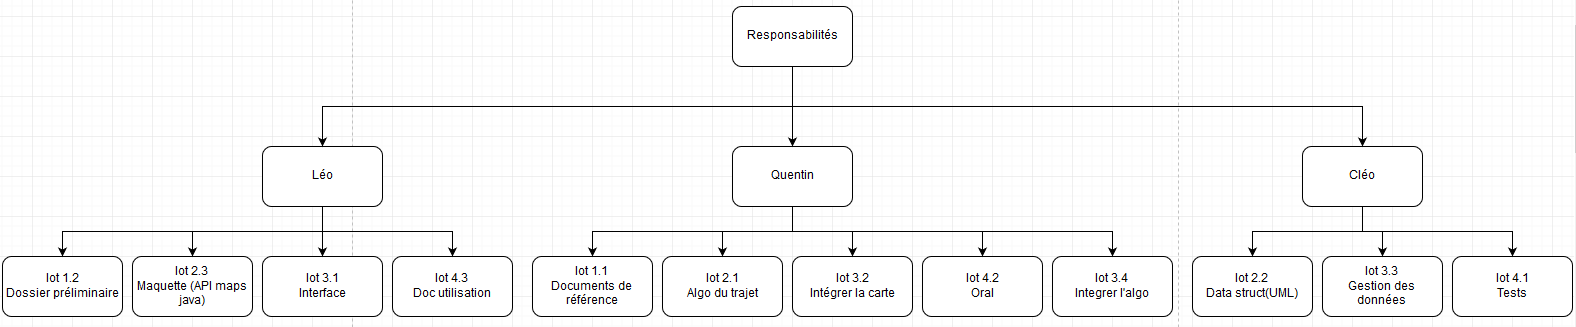
\includegraphics[angle=90, height=0.9\textheight]{img/diag-responsabilites}
\end{multicols}

\jisec{Matrice RACI}
\begin{table}[h]
\label{tab:raci}
\begin{center}
\begin{tabular}{|r l|c|c|c|}
\hline
\textbf{Lot} & \textbf{Sous-lot} & \textbf{Cléo} & \textbf{Léo} & \textbf{Quentin}\\\hline
1 & 1.1 & A  & A  & RA \\\hline
  & 1.2 & A  & RA & A  \\\hline
2 & 2.1 &    &    & RA \\\hline
  & 2.2 & RA &    & I  \\\hline
  & 2.3 & C  & RA & C  \\\hline
3 & 3.1 & IC & RA & I  \\\hline
  & 3.2 &    & C  & R  \\\hline
  & 3.3 & RA & I  &    \\\hline
  & 3.4 &    & IC & RA \\\hline
4 & 4.1 & RA & C  & C  \\\hline
  & 4.2 & A  & A  & RA \\\hline
  & 4.3 & C  & RA & C  \\\hline
\end{tabular}
\end{center}
\caption{Matrice RACI pour X Facteur}
\end{table}

\jisec{Marge libre et marge totale}
\begin{table}[h]
\label{tab:marges}
\begin{center}
\begin{tabular}{|r l|c|c|}
\hline
\textbf{Lot} & \textbf{Sous-lot} & \textbf{Marge libre} & \textbf{Marge totale}\\\hline
1 & 1.1 & 0 & 0\\\hline
  & 1.2 & 0 & 0\\\hline
2 & 2.1 & 1 & 1\\\hline
  & 2.2 & 4 & 4\\\hline
  & 2.3 & 0 & 0\\\hline
3 & 3.1 & 0 & 0\\\hline
  & 3.2 & 1 & 1\\\hline
  & 3.3 & 1 & 1\\\hline
  & 3.4 & 0 & 0\\\hline
4 & 4.1 & 0 & 0\\\hline
  & 4.2 & 0 & 0\\\hline
  & 4.3 & 0 & 0\\\hline
\end{tabular}
\end{center}
\caption{Marge libre et marge totale pour X Facteur}
\end{table}


\clearpage
\jisec{PERT}
\begin{center}
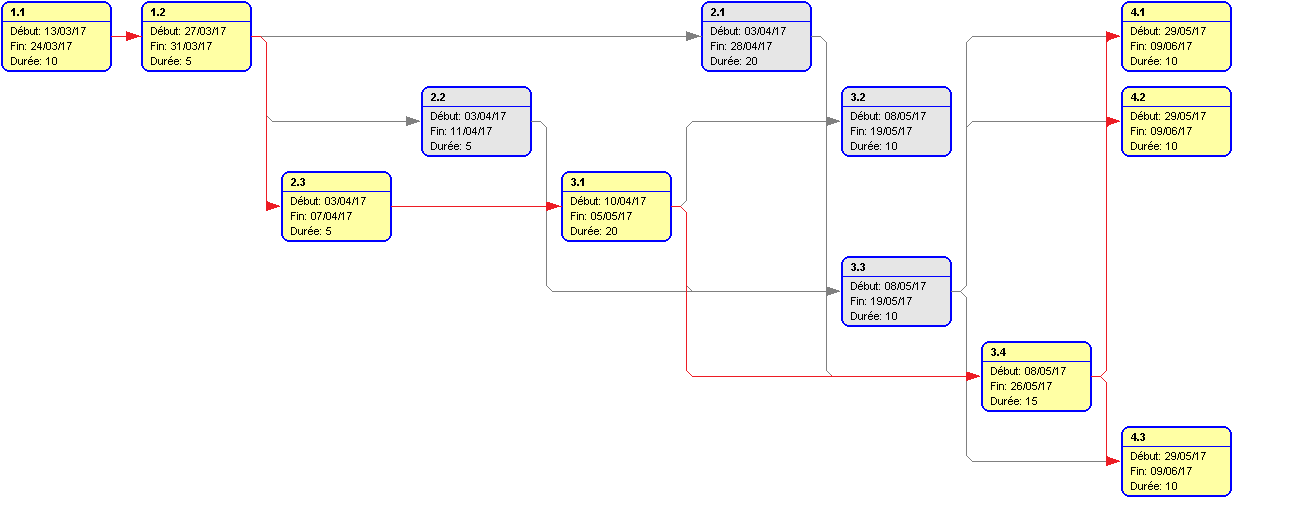
\includegraphics[angle=90, height=0.9\textheight]{img/pert.png}
\end{center}

\clearpage
\jisec{Gantt}
\begin{center}
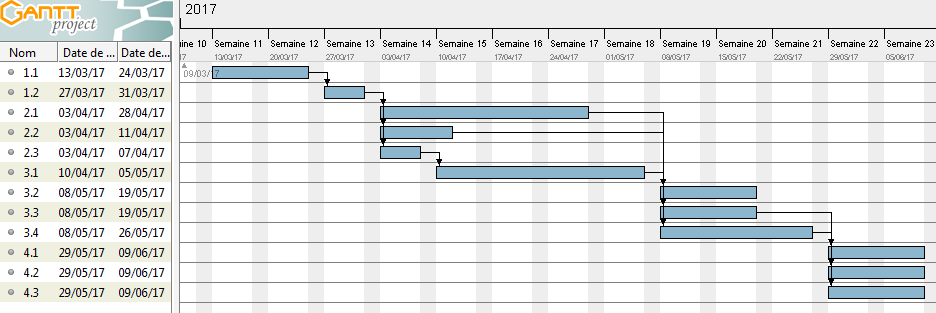
\includegraphics[angle=90, height=0.9\textheight]{img/gantt.png}
\end{center}

\end{document}
